\input{preambuloSimple.tex}

%----------------------------------------------------------------------------------------
%	TÍTULO Y DATOS DEL ALUMNO
%----------------------------------------------------------------------------------------

\title{
\normalfont \normalsize
\texttt{{\bf Visión Por Computador (2015-2016)} \\ Grado en Ingeniería Informática \\ Universidad de Granada} \\ [25pt] % Your university, school and/or department name(s)
\horrule{0.5pt} \\[0.4cm] % Thin top horizontal rule
\huge Informe Trabajo 2 - Estimación de Homografías y Construcción de panoramas \\ % The assignment title
\horrule{2pt} \\[0.5cm] % Thick bottom horizontal rule
}

\author{Mª Cristina Heredia Gómez} % Nombre y apellidos

\date{\normalsize\today} % Incluye la fecha actual

%----------------------------------------------------------------------------------------
% DOCUMENTO
%----------------------------------------------------------------------------------------

\begin{document}

\maketitle % Muestra el Título

\newpage %inserta un salto de página

\tableofcontents % para generar el índice de contenidos

\listoffigures

%\listoftables

\newpage

%NOTA: en caso de problema al compilar, compruebe que tiene el paquete: texlive-babel-spanish.noarch  \\


\newpage

%----------------------------------------------------------------------------------------
%	Ejercicio1
%----------------------------------------------------------------------------------------
\section{Estimación de una homografía: Usar las imágenes tablero1 y tablero2
incluidas en el fichero de datos para estimar la homografía que relaciona
ambas imágenes. (2.5 puntos) \newline
Para ello realizar lo siguiente: \newline
1.- Seleccionar a mano un conjunto de 10 puntos en correspondencias
en ambas imágenes (distribuir dichos puntos de la forma más uniforme posible
entre los puntos esquina del tablero). \newline
2.- Estimar la homografía (implementar código propio, SIN usar
findHomography()) definida entre las imágenes por las parejas de puntos
seleccionados \newline
3.-Usar la función warpPerspective() para generar a partir de una de las
imágenes y la homografía estimada, la otra imagen. Comentar el resultado
obtenido en comparación con la imagen original. \newline
4.- Repetir los puntos anteriores pero seleccionando nuevos 10 puntos,
en este caso todos extraídos de 3 cuadrados contiguos de una misma esquina.
Comparar el resultado obtenidos con el anterior y valorar las diferencias
encontradas.}

Tenemos:
\[\begin{pmatrix} u\\ v\\ w \end{pmatrix}=H\begin{pmatrix} x\\ y\\ 1 \end{pmatrix}\Rightarrow \begin{pmatrix} u\\ v\\ w \end{pmatrix}=\begin{pmatrix} h_{1}x& +h_{2}y &+h_{3} \\ h_{4}x& +h_{5}y &+h_{6} \\ h_{7}x& +h_{8}y & +h_{9} \end{pmatrix}\]
donde \[ X=\begin{pmatrix} x\\ y\\ 1 \end{pmatrix} \] y sabemos que $u=\frac{x1}{x3}$ y que $u=\frac{x2}{x3}$ ,donde $x1$ es la fila 1 de Xh. Luego tenemos que:
\[u=\frac{h_{1}x+h_{2}y+h_{3}}{h_{7}x+h_{8}y+h_{9}}\]
$\Rightarrow$ \[u(h_{7}x+h_{8}y+h_{9})-(h_{1}x+h_{2}y+h_{3})=0\]
y análogamente:
\[v=\frac{h_{4}x+h_{5}y+h_{6}}{h_{7}x+h_{8}y+h_{9}}\]
$\Rightarrow$ \[v(h_{7}x+h_{8}y+h_{9})-h_{4}x-h_{5}y-h_{6}=0\]
que escribiéndolo matricialmente, queda como:
\[A_{i}=\bigl(\begin{smallmatrix} -x&-y &-1 &0 &0 &0 &ux &uy &u \\ 0& 0& 0&-x &-y &-1 &vx &vy &v \end{smallmatrix}\bigr)\]
y si juntamos cada $A_{i}$ obtenemos A ,tal que $ A \cdot h=0$ donde \[h=\begin{pmatrix} h_{1} &h_{2} & h_{3} &h_{4} &h_{5} &h_{6} &h_{7} &h_{8} &h_{9} \end{pmatrix}^{T}\]

Pues bien, la idea para implementar el algoritmo que estima la homografía no ha sido más que esta. Calculamos
lo que sería la matriz A, que tendrá tantas filas como número de puntos por dos, ya que por cada punto se añaden dos filas,
y tendrá 9 columnas. \newline
Para ello, mi función recibe la imágen original y dos vectores de puntos. Unvector pertenece a la imágen original y el otro son puntos
de la imágen que queremos estimar. \newline
 Luego, con un bucle sencillo vamos calculando para cada pareja de puntos, sus dos filas de $A_{i}$. Finalmente, cuando
ya tenemos A completa, descomponemos en valores singulares la matriz A,llamando a la función \textbf{SVD} de OpenCV que hace justo eso,
y paśandole la opción \textbf{MODIFY\_A} para que modifique A directamente y así ahorrarnos hacer una copia. \newline
Hecho todo esto ya sólo hay que tomar el autovalor que hay en la posición 8, pues como sabemos
la 8 es la posición última y ahí es donde se encuentra el valor mínimo. \newline
Inicialmente, tomamos 10 puntos distribidos por el tablero. Yo lo he hecho en el main y he usado la stl para ello:
\myCppCode{CV_Practica2/main}{main}{21}{48}
Una vez que tenemos los puntos, solo queda estimar la homografía y aplicar la transformación de perspectiva a la imágen 1.
Para estimar la homografía, he implementado la siguiente función:
\myCppCode{CV_Practica2/funciones}{funciones}{30}{76}
y vemos en el resultado que nos calcula una homografía con algunos bordes negros, pero por lo general, bastante similar al Tablero2, a partir
del tablero1:
\begin{figure}[H] %con el [H] le obligamos a situar aquí la figura
\centering
\includegraphics[scale=0.3]{hcalculada.png}  %el parámetro scale permite agrandar o achicar la imagen. En el nombre de archivo puede especificar directorios
\label{figura1}
\caption{Tablero1 y homografía calculada  }
\end{figure}

\begin{figure}[H] %con el [H] le obligamos a situar aquí la figura
\centering
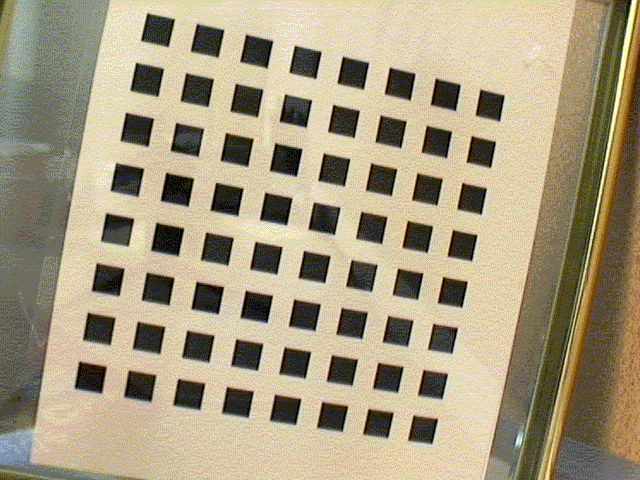
\includegraphics[scale=0.3]{Tablero2.jpg}  %el parámetro scale permite agrandar o achicar la imagen. En el nombre de archivo puede especificar directorios
\label{figura1}
\caption{imágen Tablero2.jpg original}
\end{figure}

%------------------------------------------------
%\bibliography{citas} %archivo citas.bib que contiene las entradas
%\bibliographystyle{plain} % hay varias formas de citar

%\chapter*{Bibliograf\'ia}
%\section*{Referencias}
%\addcontentsline{toc}{section}{Articles}
%\printbibliography[heading=bibempty,type=article]
%\printbibliography[heading=bibempty,type=misc]
\end{document}
